\section{Terrain following stable atmosphere advection}

\TODO{theta contours?  theta diff heatmap?  l2 error norm?}

\begin{figure}
	\captionsetup[subfigure]{position=b}
	\centering
	\subcaptionbox{BTF \label{fig:wobblyThetaAdvection:thetaDiff:btf}}[0.49\textwidth]{\includegraphics[height=2.6in,angle=270]{openfoam/cases/wobblyThetaAdvection/btf/schaerExp/cubicUpwindCPCFit/18000/thetaDiff.eps}}
	\hfill
	\subcaptionbox{SnapCol \label{fig:wobblyThetaAdvection:thetaDiff:snapCol}}[0.49\textwidth]{\includegraphics[height=2.6in,angle=270]{openfoam/cases/wobblyThetaAdvection/snapCol/schaerExp/cubicUpwindCPCFit/18000/thetaDiff.eps}}
%
	\caption{\TODO{theta diff heatmap} \TODO{colour legend}}
	\label{fig:wobblyThetaAdvection:thetaDiff}
\end{figure}

\begin{align}
\frac{\partial h}{\partial x} &= - 2 h_0 \exp \left( - \left( \frac{x}{a} \right)^2 \right) \cos \left( \frac{\pi x}{\lambda} \right) \left[
\frac{\pi}{\lambda} \sin \left(\frac{\pi x}{\lambda} \right) +
\frac{x}{a^2} \cos \left( \frac{\pi x}{\lambda} \right) \right]
\end{align}
